\begin{figure}[hbtp]
    \centering
    %\scriptsize
    % \setstretch{0.9}
    \begin{subfigure}{0.49\textwidth}
        % \def\svgwidth{9.0cm}
        \includegraphics[width=0.95\textwidth]{3_modeling/figures/DUAL.pdf}
        \caption{CMOS inverter in a dual-well silicon substrate sectional view. The epitaxy is the junction between the P-substrate and the N-well. $RC_{GND}$ is the access resistance from the epitaxy to the NMOS through the P-substrate. $RC_{VDD}$ is the access resistance from the epitaxy to the PMOS through the N-well.}
        \label{subfig:dualIvx}
    \end{subfigure}
    \hfill
    \begin{subfigure}{0.49\textwidth}
        % \def\svgwidth{9.0cm}
        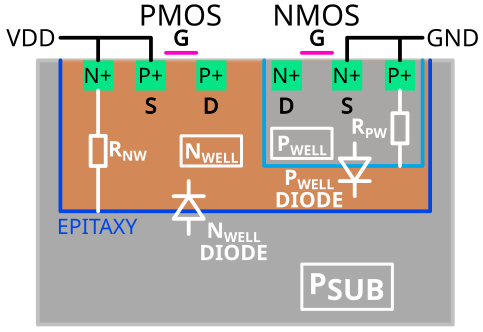
\includegraphics[width=0.95\textwidth]{3_modeling/figures/TRIPLE.pdf}
        \caption{CMOS inverter in a triple-well silicon substrate sectional view. The epitaxy is the junction between the P-substrate and the N-well. $R_{NW}$ is the access resistance from the epitaxy to the PMOS through the N-well. Inside the N-well is created the P-well. $R_{PW}$ is the access resistance from the N-well/P-well junction to the NMOS.}
        \label{subfig:tripleIvx}
    \end{subfigure}
    \caption{Dual-well (\ref{subfig:dualIvx}) and triple-well (\ref{subfig:tripleIvx}) inverter silicon sectional view.}
    \label{fig:dualTripleIvx}
\end{figure}